% Объединение возможностей
\label{collective_global}

Если оценку параметров объектов $x_{ij}$ совершают несколько экспертов, исходным материалом для программного комплекса служат оценки 
\begin{equation}
\label{Psetlargedef}
	\Pi = \{\p_{ij}^{(r)}\}, i = \dotN, j = \dotM, r = \dotR, 
\end{equation}
где $r$ --- номер эксперта. На вход алгоритма выбора объектов подаются только экспертное  мнение одного эксперта (см. рис.~\ref{ris:program_global}): 
\begin{equation*}
	\Pi* = \{\p_{ij}\},  i = \dotN, j = \dotM,
\end{equation*}		
 поэтому в настоящем разделе ставятся задачи сведения набора $\Pi$ к $\Pi*$ --- задачи нахождения  оценки, выражающей коллективное мнение экспертов, или, короче говоря, задачи <<коллективной экспертизы>>. 

\begin{figure}[h]
\center{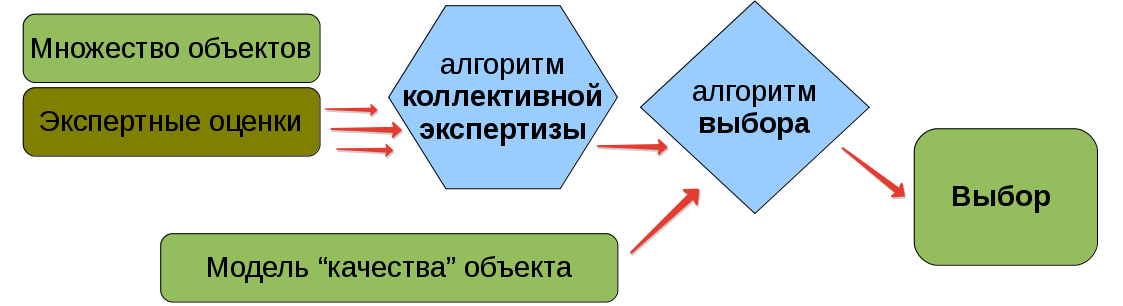
\includegraphics[width=0.85\linewidth]{./pic/globalscheme}}  
\caption{\small Схема, иллюстрирующая работу программного комплекса в режиме нахождения наиболее <<качественных>> объектов на выходе по мнениям нескольких экспертов и модели <<качества>> объектов (функции $f: x = f(x_1, x_2, ...)$) на входе. }
\label{ris:program_global}
\end{figure}

Задача коллективной экспертизы в рамках использования модели нечётких оценок в теории возможностей Пытьева может быть поставлена и решена различными методами:
	\begin{enumerate}
		\item Методы <<евклидовой близости к среднему>>~\cite{pytyev_experts}: метод матриц попарных сравнений, векторов перестановок, векторов предпочтений и др.;
		\item Новый (в рамках теории возможности Пытьева) метод -- метод векторов предпочтений;
		\item Новый метод -- введение отношения квазипорядка~\ref{preorder_pyt}  на множестве распределений нечёткого элемента и вычисление верхней грани (или  точной верхней грани) распределений~\ref{Psetlargedef}.
	\end{enumerate} 
	
\subsection{Метод матриц попарных сравнений}


\subsection{Метод векторов предпочтений}


\subsection{Метод вычисления верхней грани распределений на входе}


	
	